\MindQuantum\ 非常重视 NISQ 算法的模拟效率，尤其是变分量子算法的模拟效率。本节将 \MindQuantum\ 与其他量子计算框架进行基准测试。首先，我们使用随机线路模拟来评估框架的基础性能。其次，我们使用量子近似优化算法（QAOA）进行基准测试，以展示 MindQuantum 解决实际问题的能力。下表列出了参与基准测试的框架。

\begin{table}[ht]
    \begin{tabular}{cc}
        \toprule
        框架          & 版本    \\
        \midrule
        MindQuantum        & 0.9.0      \\
        Qiskit             & 0.45.0     \\
        Projectq           & 0.8.0      \\
        Pennylane          & 0.33.0     \\
        PyQpanda           & 3.8.0      \\
        Qulacs             & 0.6.2      \\
        Tensorflow Quantum & 0.7.2      \\
        Intel-QS           & 2.0.0-beta \\
        Cuquantum          & 23.10.0    \\
        \bottomrule
    \end{tabular}
    \caption{基准测试所用的软件版本。}
    \label{tab:software version}
\end{table}

基准测试使用的硬件平台为 Intel$^\circledR$ Xeon$^\circledR$ CPU E5-2620 v3 @ 2.40GHz（基准测试中使用 16 个线程），启用 SIMD；GPU 为 NVIDIA-V100。基准测试框架为 pytest-benchmark。

\begin{figure*}
    \centering
    \begin{subfigure}{0.45\textwidth}
        \centering
        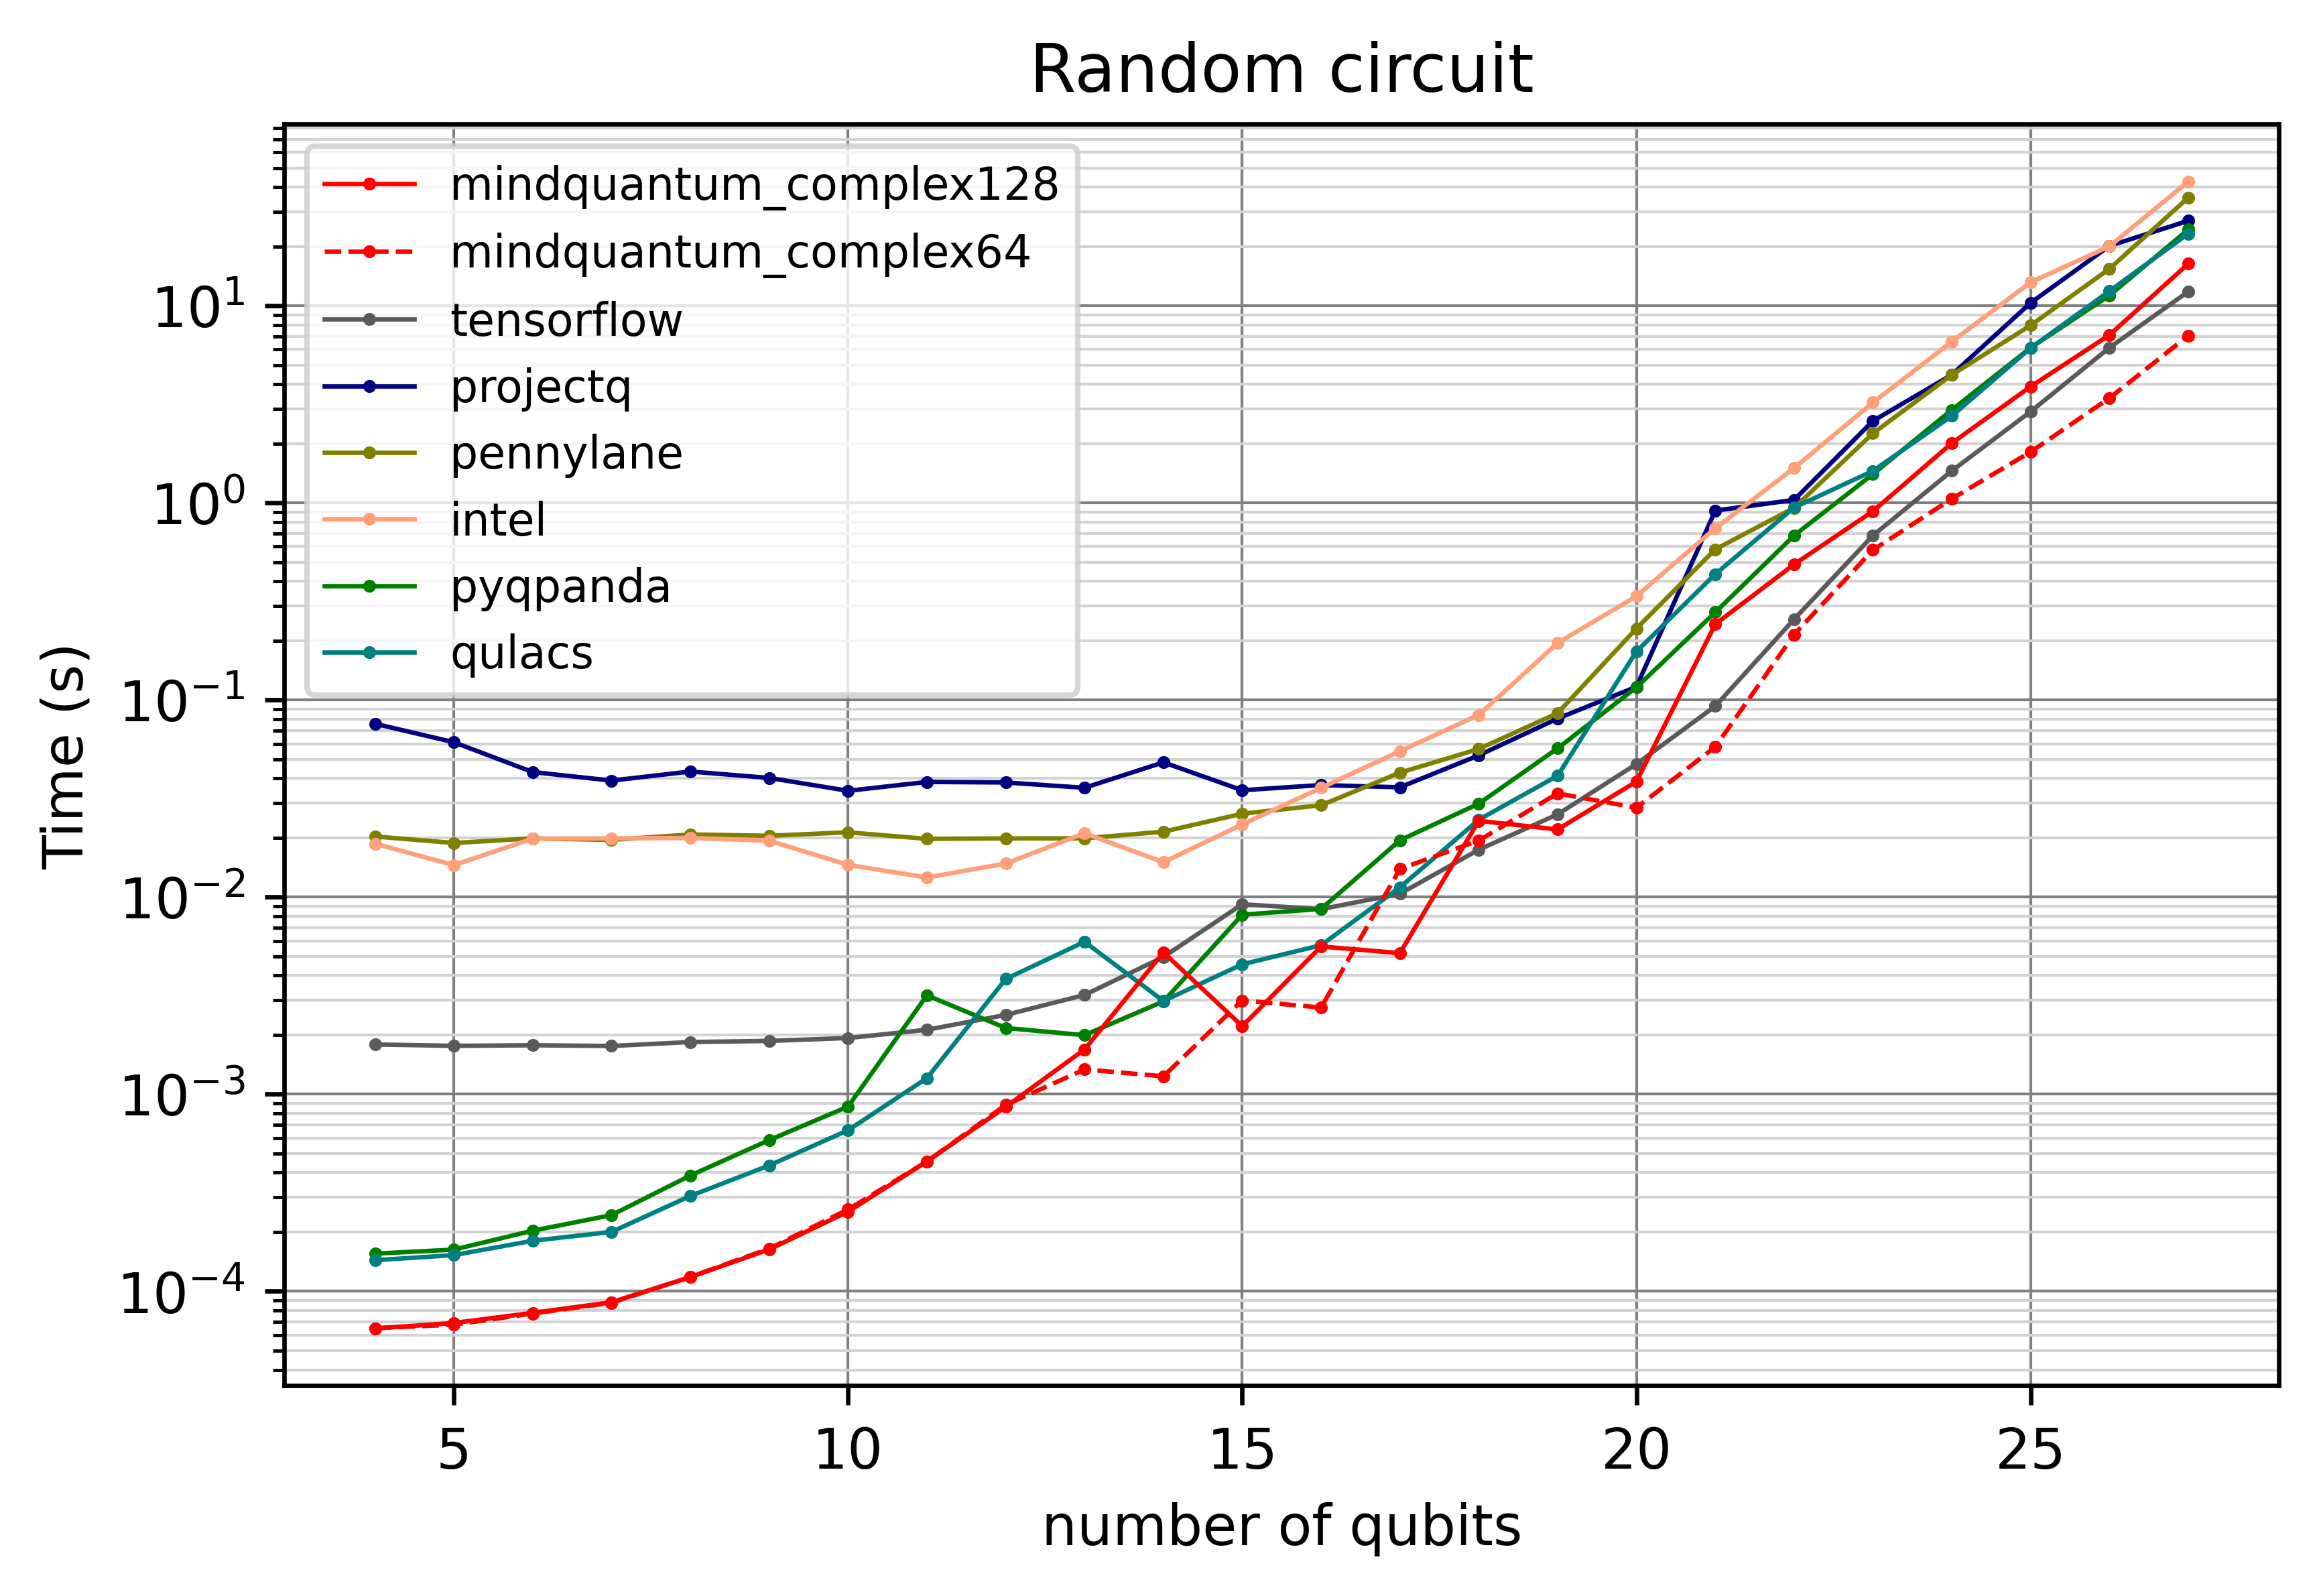
\includegraphics[width=\textwidth]{images/7_Random_circuit_CPU.png}
        \caption{CPU 后端上的随机线路基准测试。}
        \label{7_random_circ_cpu}
    \end{subfigure}
    \begin{subfigure}{0.45\textwidth}
        \centering
        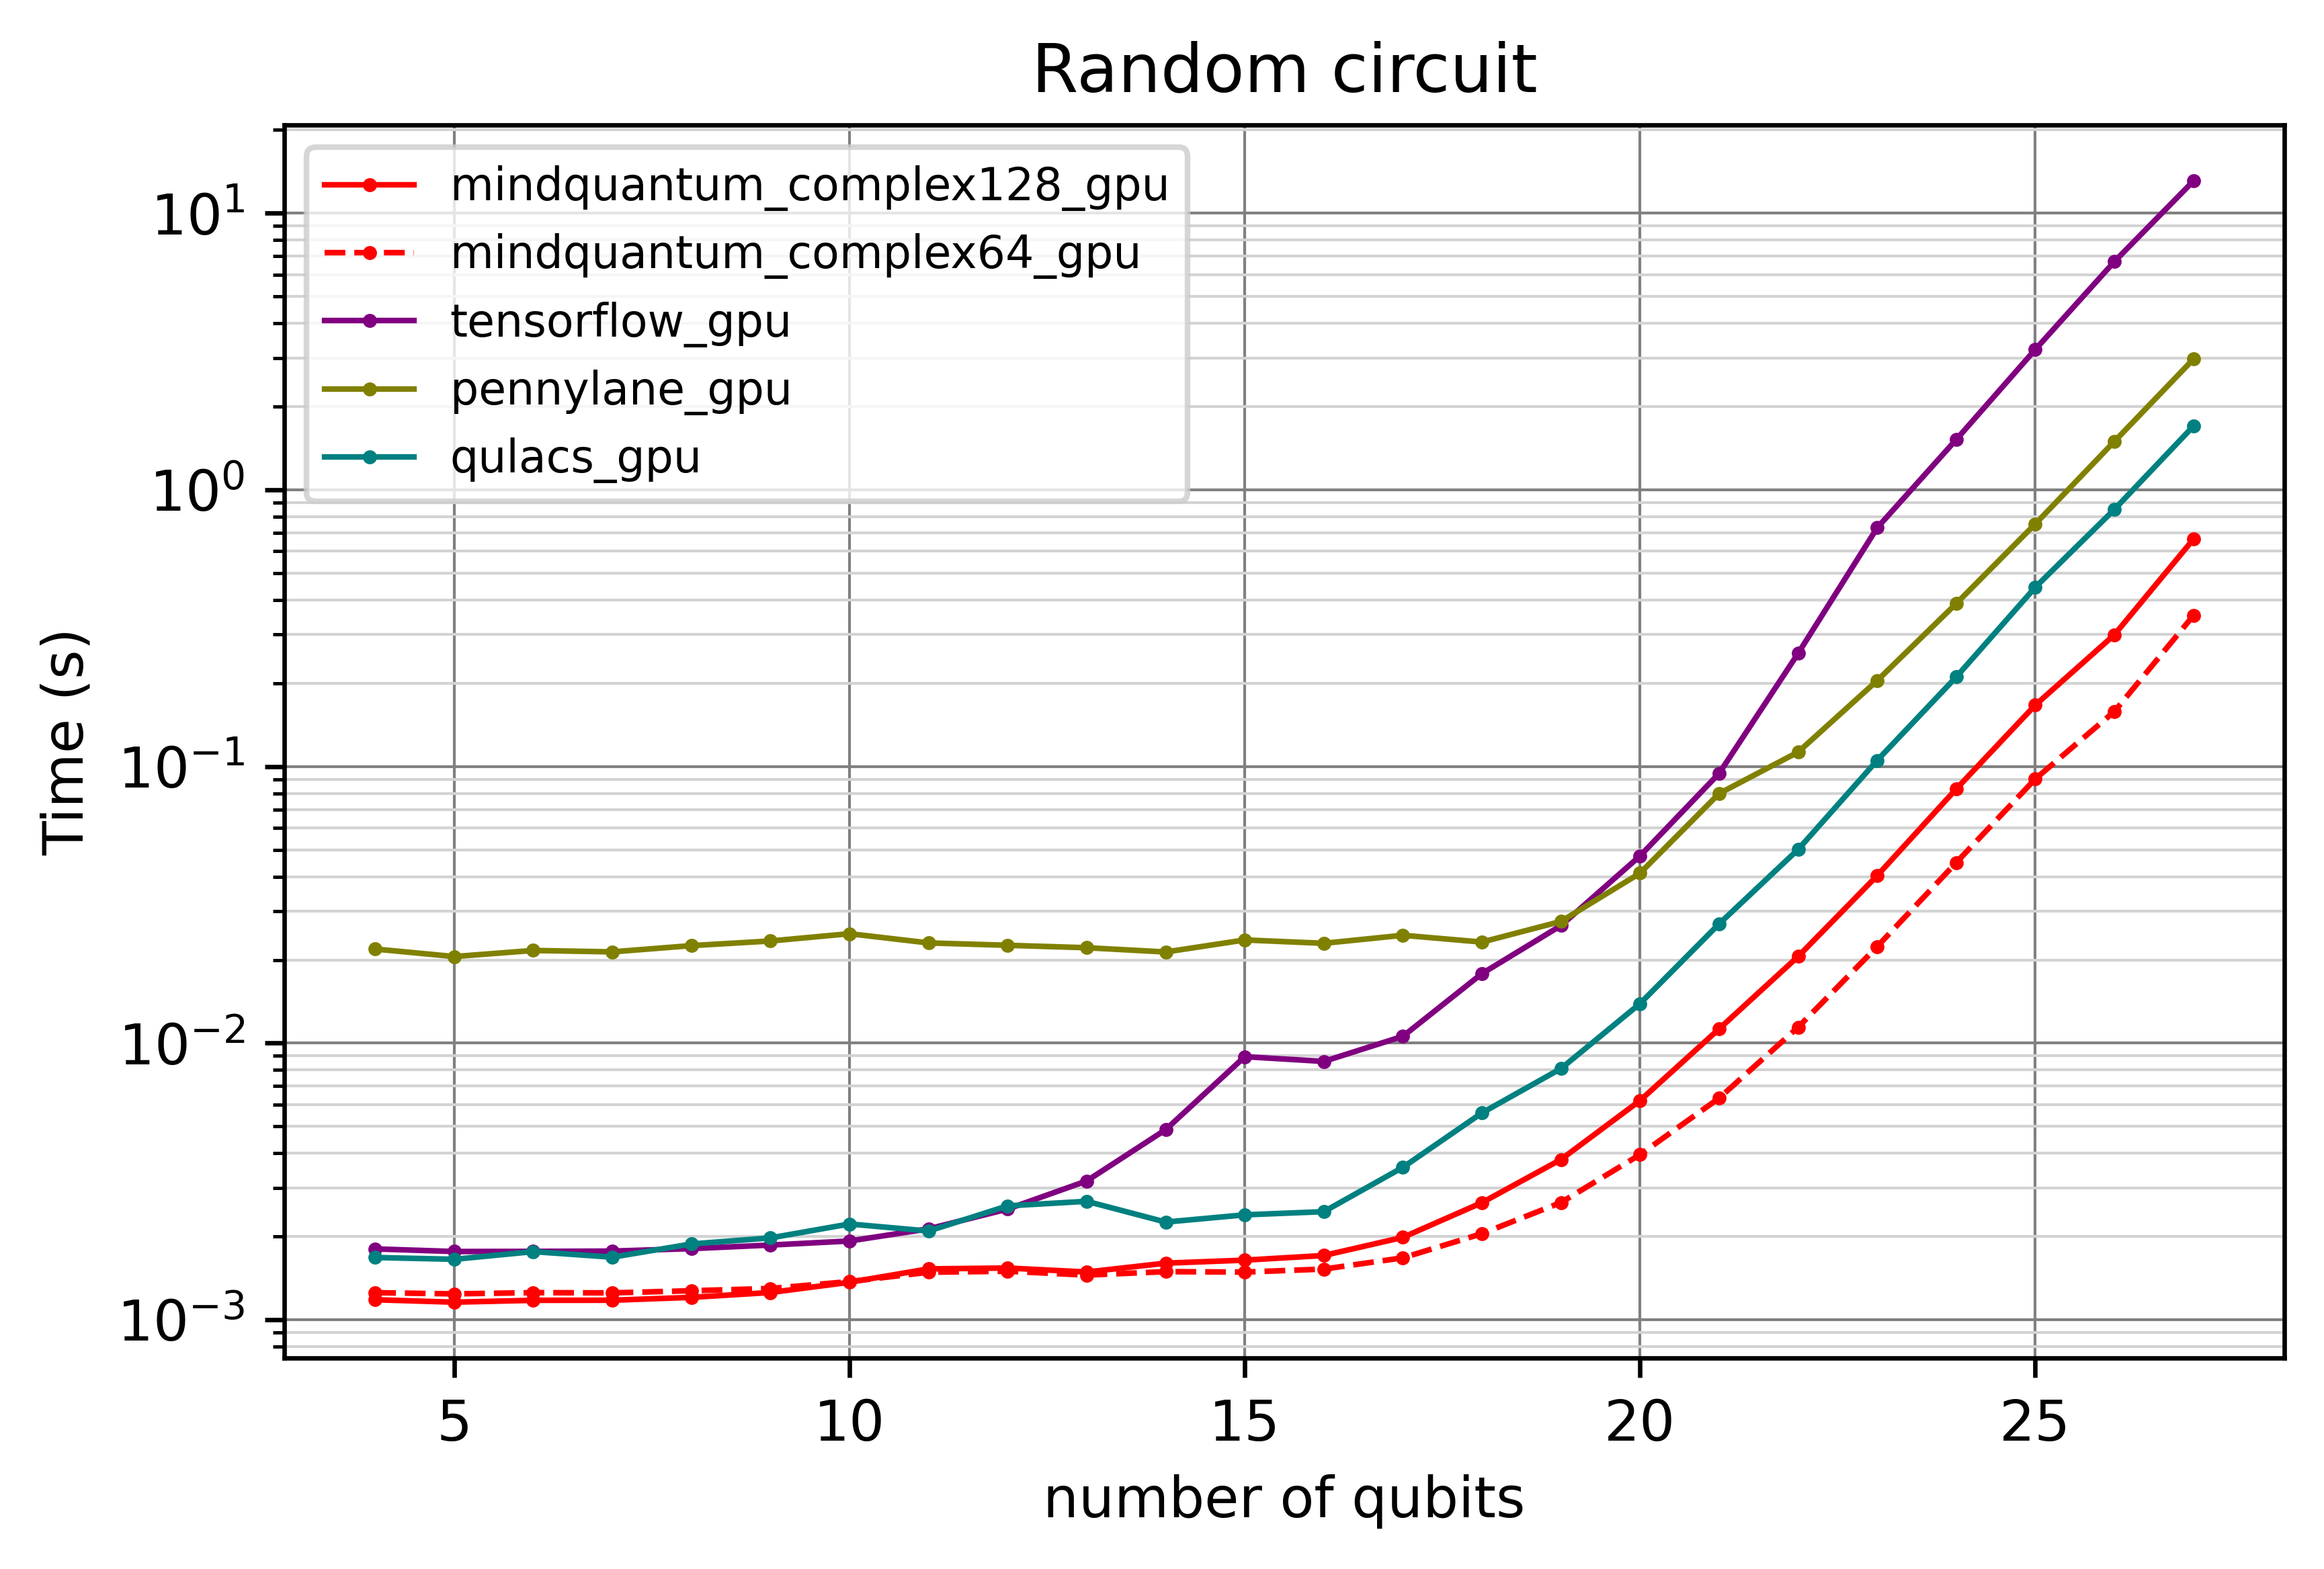
\includegraphics[width=\textwidth]{images/7_Random_circuit_GPU.png}
        \caption{GPU 后端上的随机线路基准测试。}
        \label{7_random_circ_gpu}
    \end{subfigure}
    \begin{subfigure}{0.45\textwidth}
        \centering
        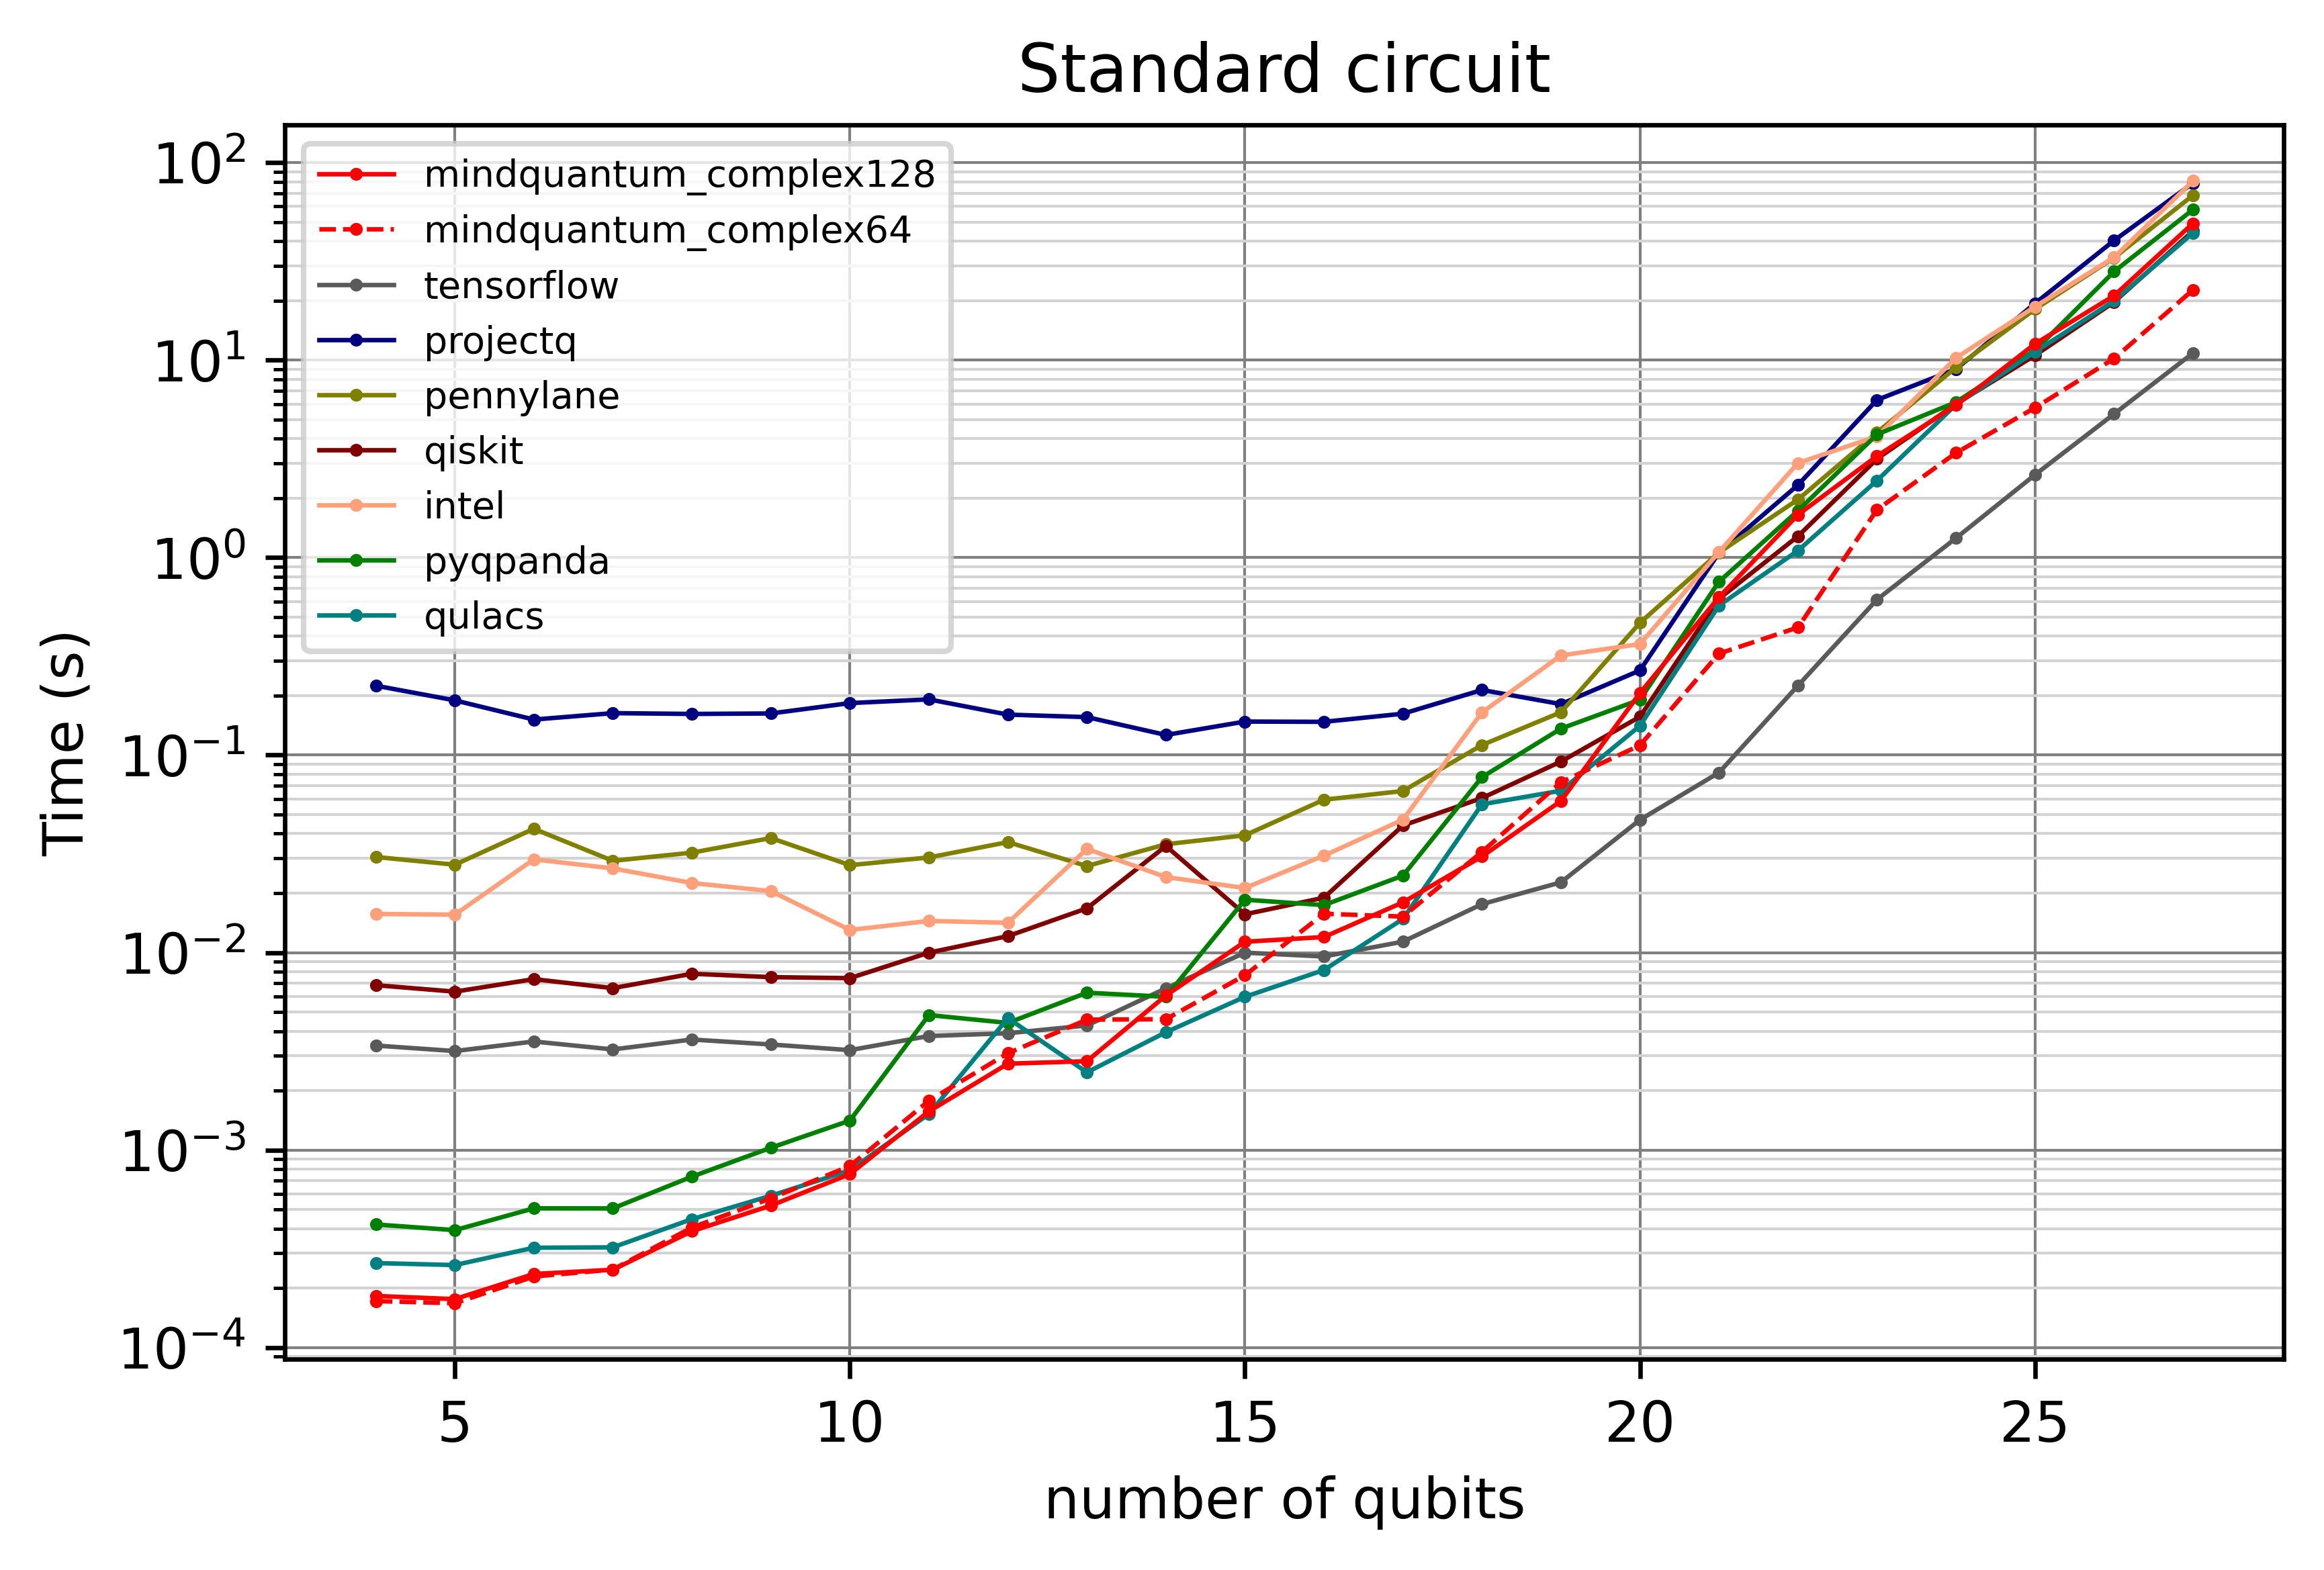
\includegraphics[width=\textwidth]{images/7_Simple_circuit_CPU.png}
        \caption{CPU 后端上的标准线路基准测试。}
        \label{7_simple_circ_cpu}
    \end{subfigure}
    \begin{subfigure}{0.45\textwidth}
        \centering
        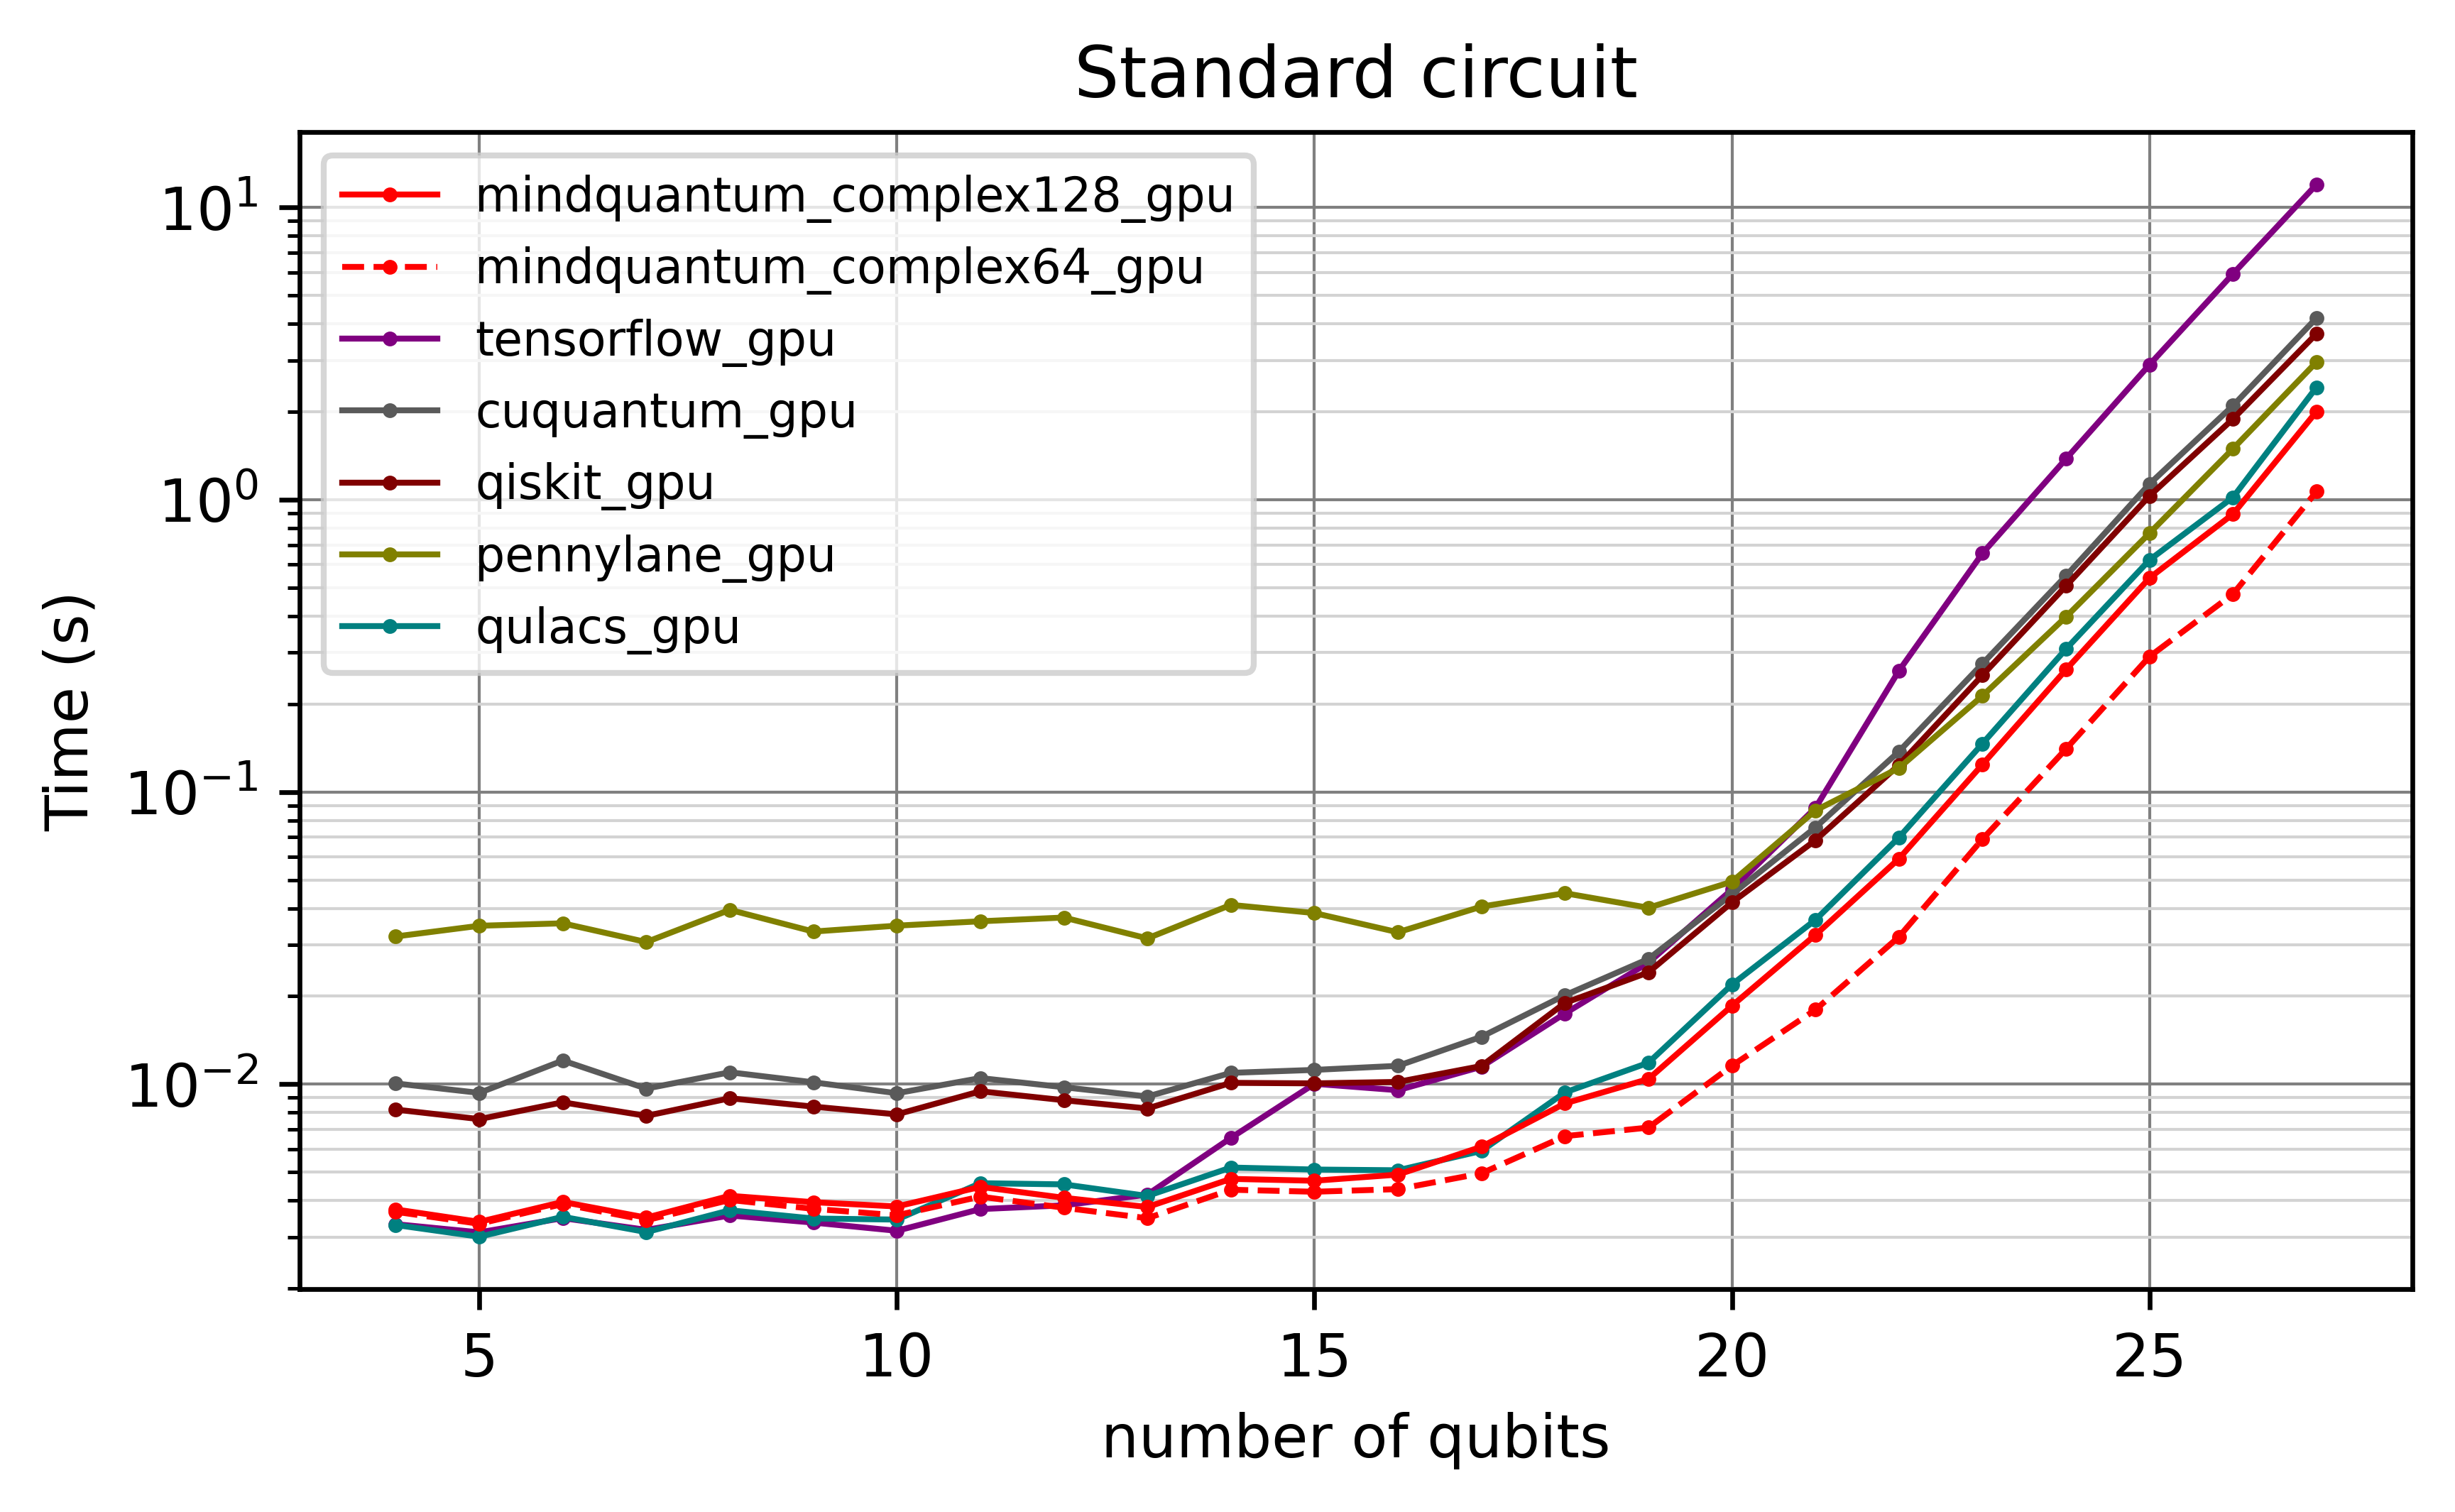
\includegraphics[width=\textwidth]{images/7_Simple_circuit_GPU.png}
        \caption{GPU 后端上的标准线路基准测试。}
        \label{7_simple_circ_gpu}
    \end{subfigure}
    \caption{不同后端上随机复杂线路与随机简单线路的基准测试。}
    \label{fig:benchmark_circ}
\end{figure*}

\subsection{运行随机线路任务}

在随机线路基准测试中，我们选择两类不同线路。第一类任务是复杂随机线路，量子比特数从 4 到 27 不等。复杂随机线路包含 X、Y、Z、H、CNOT、S、T、RX、RY、RZ、Rxx、Ryy、Rzz、SWAP 门及其受控版本。第二类任务是由对应复杂随机线路分解得到的简单随机线路，其中仅包含基础门集合。除 TensorFlow Quantum 外，基准测试中各模拟器均采用双精度。基准测试结果如图 \ref{fig:benchmark_circ} 所示。


总体而言，模拟时间会随线路规模呈指数增长。然而，当量子比特数较小时，\MindQuantum、Qulacs 和 Qpanda 在耗时方面相较其他框架具有明显优势，这主要来自 API 调用开销的差异。值得注意的是，在 13 量子比特位置附近出现了轻微下降，这是因为 \MindQuantum\ 以 13 个量子比特作为阈值；当量子比特数大于 13 时，会启用 OpenMP 进行多线程并行计算，否则使用单线程模拟。这样设计的原因是，当量子比特数较小时，多线程计算反而会降低运行速度。随着线路规模继续增大，\MindQuantum\ 和 Qulacs 保持了良好的速度优势，可以判断这两个框架在底层实现上已经优化到接近极限。在处理大比特数简单线路时，TensorFlow Quantum 表现出优势，原因有两点：第一，它采用单精度计算；第二，它针对基础量子门加入了更多专门优化。

\begin{figure*}
    \centering
    \begin{subfigure}{0.9\textwidth}
        \centering
        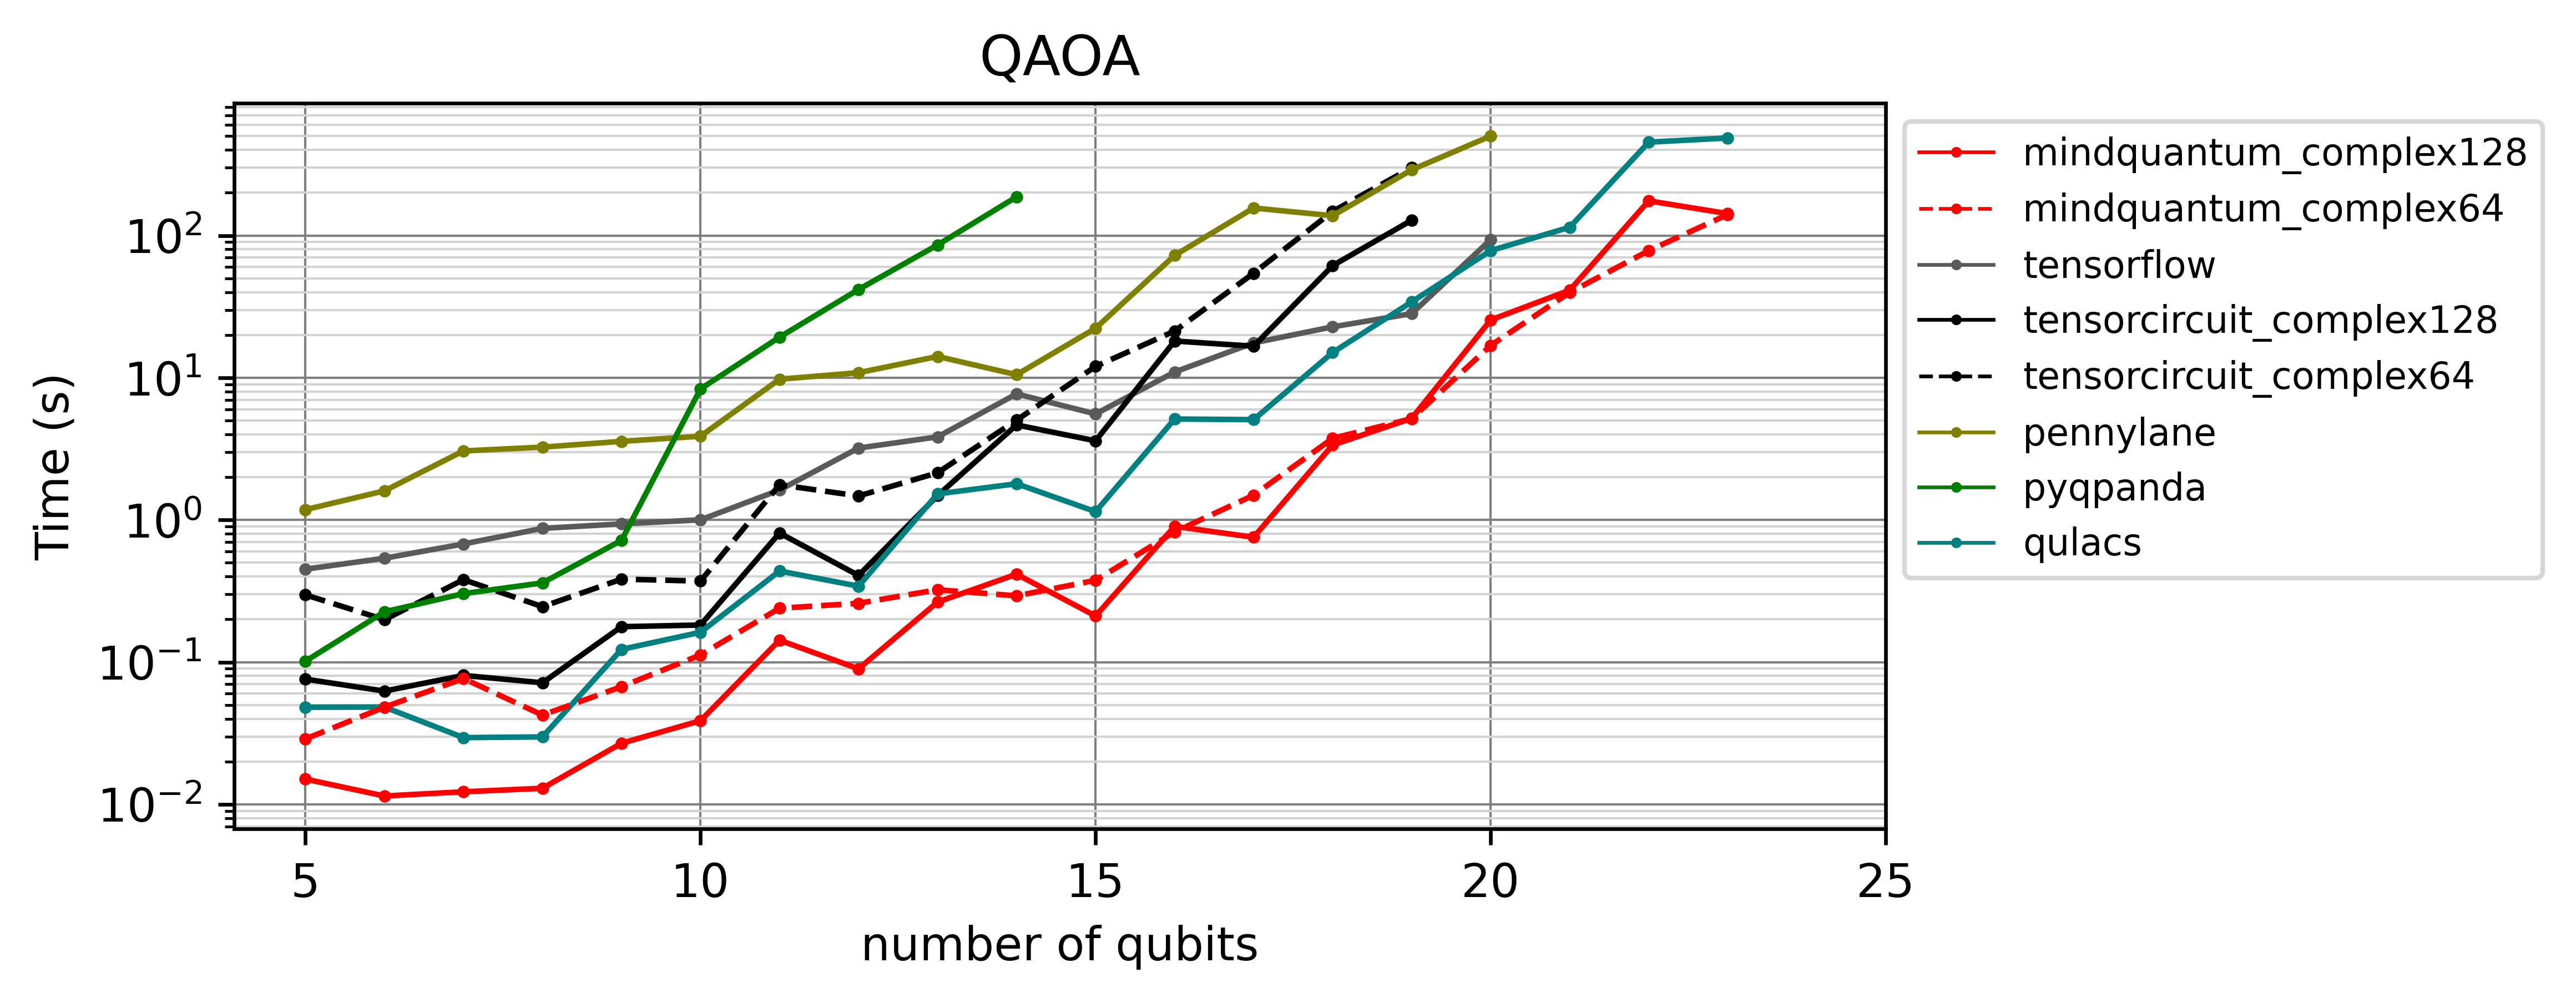
\includegraphics[width=\textwidth]{images/7_QAOA_CPU.png}
        \caption{CPU 上 4-正则图 QAOA 端到端优化基准测试。}
        \label{7_regular_4_cpu}
    \end{subfigure}
    \begin{subfigure}{0.9\textwidth}
        \centering
        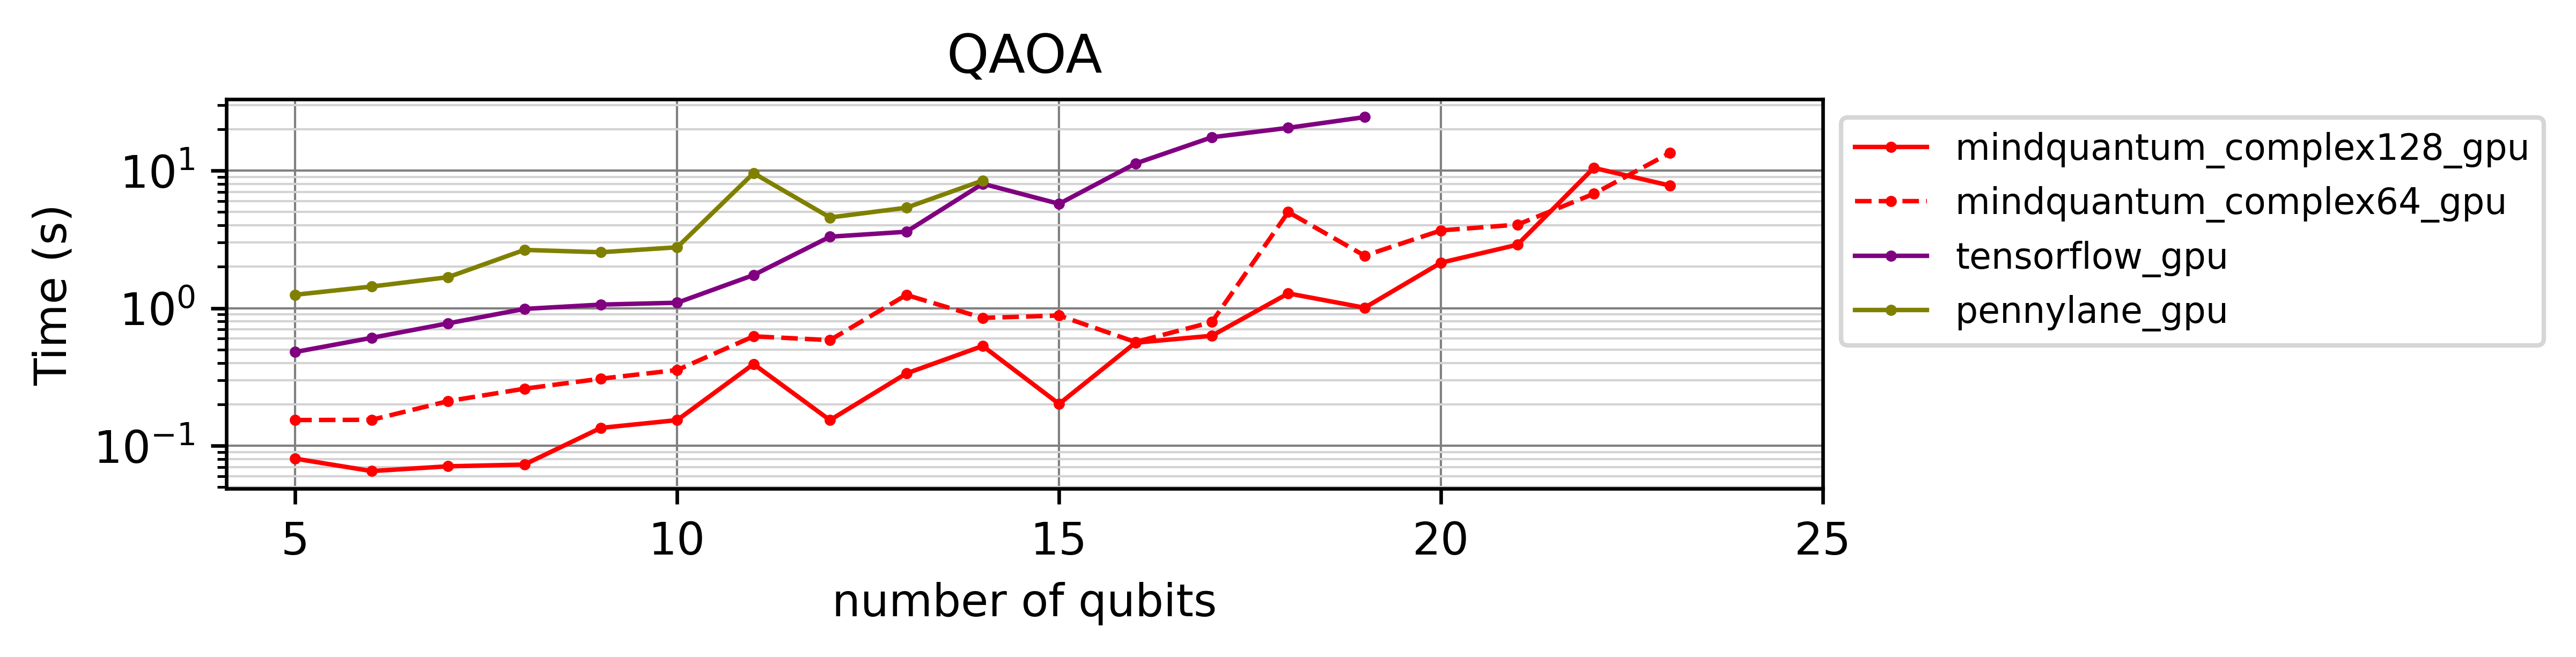
\includegraphics[width=\textwidth]{images/7_QAOA_GPU.png}
        \caption{GPU 上 4-正则图 QAOA 端到端优化基准测试。}
        \label{7_regular_4_gpu}
    \end{subfigure}
    \caption{不同后端上的 QAOA 基准测试。}
    \label{fig:benchmark_qaoa}
\end{figure*}

\subsection{QAOA 任务}

变分量子算法也是 NISQ 阶段非常重要的一类算法。在本部分中，我们选择量子近似优化算法进行基准测试，以进一步展示框架在求解实际问题时的性能。我们使用 QAOA 求解 4-正则图的最大割问题，问题规模从 5 个节点到 23 个节点不等。ansatz 线路通过一步 Trotter 分解得到。优化器采用 \code{scipy.optimize.minimize()} 中的 BFGS 方法。由于大规模 QAOA 任务耗时较长，当某个框架的运行时间达到指定阈值时，我们会停止其执行。因此，在结果图中，各框架数据点所能达到的最大量子比特数并不一致。基准测试结果如图 \ref{fig:benchmark_qaoa} 所示。

总体来看，随着问题规模增加，所有框架的求解时间都呈指数增长。然而，对于这些问题，\MindQuantum\ 相比其他框架至少快一个数量级。这主要得益于 MindQuantum 中针对参数化量子线路梯度计算优化过的伴随方法，以及高效的线路演化实现。
